\title{Historical biogeography in RevBayes}
\author{Michael J. Landis \\ \href{mailto:mlandis@berkeley.edu}{\texttt{mlandis@berkeley.edu}}}

\section{Introduction}

This lab describes how to perform Bayesian inference of historical biogeography using RevBayes. 


\subsection*{\textbf{Outline}}
\begin{tabular}{ll}
{\bf I. Introduction} & \\
& a) Workspace setup \\
& b) Range evolution models and data augmentation \\
{\bf II. DEC in RevBayes} & \\
& a) Tree, range, and geographic input \\
& b) DEC as a graphical model \\
& c) Monitors, moves, and MCMC \\
& d) Model selection with Bayes factors \\
{\bf III. Output and Analysis} & \\
& a) MCMC output in Tracer \\
& b) Ancestral range output \\
& c) Animate ancestral ranges \\
\end{tabular}

\noindent \\ \impmark These little arrows indicate lines containing key information to progress through the lab. The rest of the text gives context for why we're taking these steps or what to make of results.

\subsection{Handy links for this lab}

\begin{tabular}{ll}
RevBayes & \url{https://github.com/revbayes/revbayes} \\
Lab zip file & \href{https://github.com/revbayes/revbayes/raw/development/tutorials/RB\_Biogeography\_tutorial/RB\_biogeo\_files.zip}{{\tt https://github.com/revbayes/revbayes/.../RB\_biogeo\_files.zip}} \\
Phylowood software & \url{http://mlandis.github.io/phylowood} \\
Phylowood manual & \url{https://github.com/mlandis/phylowood/wiki} \\
Tracer & \url{http://tree.bio.ed.ac.uk/software/tracer}
%DendroPy manual & \url{http://pythonhosted.org/DendroPy/} \\
%matplotlib manual & \url{http://matplotlib.org/} \\
%NumPy manual & \url{http://www.numpy.org/}

\end{tabular}

\subsection{Setting up your workspace}

The practical part of the lab will analyze a small dataset of 19 taxa distributed over 4 biogeographic areas.
Parts of the lab will require entering terminal commands, which will assume you are using the Unix shell \texttt{bash}.
Just ask for help if the commands don't seem to work.

\noindent \\ \impmark Portions of this lab require Python is installed. No packages are needed.

\noindent \\ \impmark This tutorial will assume you have successfully installed RevBayes and can be called from your current working directory.

\noindent \\ \impmark Download and unzip the lab zip file, {\tt RB\_biogeo\_files.zip}.

%%%%%%%%%%%%%%%%
%%%%%%%%%%%%%%%%

\subsection{Motivation}

XXX

\subsection{Model and method}

This section contains a brief description of the data, model, parameters, and method used in BayArea.

First, we define the range for taxon $i$ as the bit vector $X_i$, where $X_{i,j} = 1$ if the taxon is present in area $j$ and $X_{i,j} = 0$ if the taxon is absent.
Each taxon range is a bit vector of length $N$ areas.
For example, if taxon $B$ is present only in areas 2 and 3 out of $N=3$ areas, its range is represented as $X_B = (0,1,1)$, which is translated to the bit string $X_B=011$ for short.
If we apply the labels A, B, and C to our three areas, this bit vector can also be represented as a set: $X_B=011$ is the same as $X_B = \{ B, C \}$, or $X_B=BC$ for short.
The data matrix, $\textbf{X}$, is analogous to a multiple sequence alignment where each element in the data matrix reports a discrete value for a homologous character shared by all taxa at column $j$.

\section{Modeling anagenic range evolution}

Next, we need a model of anagenic range evolution.
Since we have discrete characters we'll use the continuous-time Markov chain, which allows us to compute transition probability of a character changing from $i$ to $j$ in time $t$ through matrix exponentiation
\[
\mathbf{P}_{i,j}(t) = \left[ \exp \left\lbrace \mathbf{Q}t \right\rbrace \right]_{i,j},
\]
where $\textbf{Q}$ is the instantaneous rate matrix defining the rates of change between all pairs of characters, and $\textbf{P}$ is the transition probability rate matrix.
This technique of matrix exponentiation is powerful because it integrates over all possible scenarios of character transitions that could occur during $t$ so long as the chain begins in state $i$ and ends in state $j$. Remember, $i$ and $j$ represent different ranges, each of which is encoded as a set of occupied areas.

We can then encode range evolution events into the allowed character transitions of $\textbf{Q}$ and parameterize the events so that we may infer their relative importance to generating our observed ranges.
We'll take a simple model of range expansion (e.g. $BC \rightarrow ABC$) and range contraction (e.g. $BC \rightarrow C$).
(Range expansion may also be referred to as dispersal or area gain and range contraction as extirpation or area loss.)
The rates in the transition matrix for three areas might appear as

\[
\textbf{Q} = 
	\begin{array}{c|cccccccc}
		& \emptyset & A & B & C & AB & AC & BC & ABC \\
		\hline
		\emptyset & - & 0 & 0 & 0 & 0 & 0 & 0 & 0 \\
		A & e_A & - & 0 & 0 & d_{AB} & d_{AC} & 0 & 0 \\
		B & e_B & 0 & - & 0 & d_{BA} & 0 & d_{BC} & 0 \\
		C & e_C & 0 & 0 & - & 0 & d_{CA} & d_{CB} & 0 \\
		AB & 0 & e_B & e_A & 0 & - & 0 & 0 & d_{AC} + d_{BC} \\
		AC & 0 & e_C & 0 & e_A & 0 & - & 0 & d_{AB} + d_{CB} \\
		BC & 0 & 0 & e_C & e_B & 0 & 0 & - & d_{BA} + d_{CA} \\
		ABC & 0 & 0 & 0 & 0 & e_C & e_B & e_A & - \\								
	\end{array},
\]
where $e = ( e_A, e_B, e_C )$ are the (local) extinction rates per area, and $d = ( d_{AB}, d_{AC}, d_{BC}, d_{CB}, d_{CA}, d_{BA})$ are the dispersal rates between areas.

{\bf Q: For the three-area DEC rate matrix above, what is the rate of leaving state 101? That is, what is the absolute value of the diagonal term in the rate matrix for $Q_{AB,AB}$? }

Note the rate of more than one event occurring simultaneously is zero, so a range must expand twice by one area in order to expand by two areas.

{\bf Q: What events might explain a transition from range $ABC$ to range $A$? From range $AB$ to range $C$?}

Of course, this model can be specified for more than three areas.

{ \bf Q: Imagine a DEC rate matrix with four areas, $ABCD$. What would be the dispersal rate for $Q_{BC,BCD}$? How many states does a DEC rate matrix with four areas have? What is the relationship between the number of areas and the number of states under the DEC model? }

Let's consider what happens to the size of \textbf{Q} when the number of areas, $N$, becomes large.
For three areas, \textbf{Q} is size $8 \times 8$.
For ten areas, \textbf{Q} is size $2^{10} \times 2^{10} = 1024 \times 1024$, which approaches the largest size matrix that can be exponentiated in a practical amount of time.
For biogeographic inference under large numbers of areas, see the Tutorial XXX \citep{landis13}.



\subsection{Modeling cladogenic range evolution}

In addition to dispersal and extinction, the DEC models cladogenic range evolution events.
For each internal node in the reconstructed tree, one of two cladogenic events can occur: sympatry or allopatry.
Say the range of a species approaching an internal node, i.e. that is about to speciate, is $A$.
Since the species range is size one, this always results in sympatry, where both daughter lineages inherit the ancestral species range, so both lineages begin in state $A$.
The notation $A \rightarrow A \mid A$ describes this event: the state is $A$ before cladogenesis, the left daughter inherits range $A$ after cladogenesis, as does the right daughter.

Now suppose the ancestral range is $ABC$.
Under sympatric cladogenesis, one lineage identically inherits the ancestral species range, $ABC$, while the other lineage inherits only a single area, i.e. only $A$ or $B$ or $C$.

Under allopatric cladogenesis, the ancestral range is split evenly among daughter lineages, e.g. one lineage may inherit $AB$ and the other inherits $C$.
Both daughter lineages inherit the entire ancestral species range following widespread sympatric cladogenic events.
For a general description of state transitions for cladogenic events, see \citet{matzke13}.

{\bf Q: What are the 6 possible states in the daughter lineages after cladogenesis given the state is $AB$ before cladogenesis?}

The probabilities of anagenic change along lineages must account for all combinations of starting states and ending states.
For 3 areas, there are 8 states, and thus $8 \times 8 = 64$ probability terms for pairs of states.
For cladogenic change, we need transition probabilities for all combinations of states before cladogenesis, after cladogenesis for the left lineage, and after cladogenesis for the right lineage.
Like above, for three areas, there are 8 states, and $8 \times 8 \times 8 = 512$ cladogenic probability terms.

{\bf Q: For three areas, there are 3 + 12 + 6 = 21 possible sympatry events and 6 + 6 = 12 possible allopatry events. How many terms in the cladogenesis matrix are zero?}

The DEC model ignores speciation events hidden by extinction or incomplete taxon sampling.
The probability of cladogenesis and local extinction events would ideally be linked to a birth-death process, as it is in the GeoSSE model \citep{goldberg11}.
Unfortunately, since this sort of model scales poorly, and DEC models remain the only option when the geography has more than two or three areas.


\begin{figure}[H]
\centering
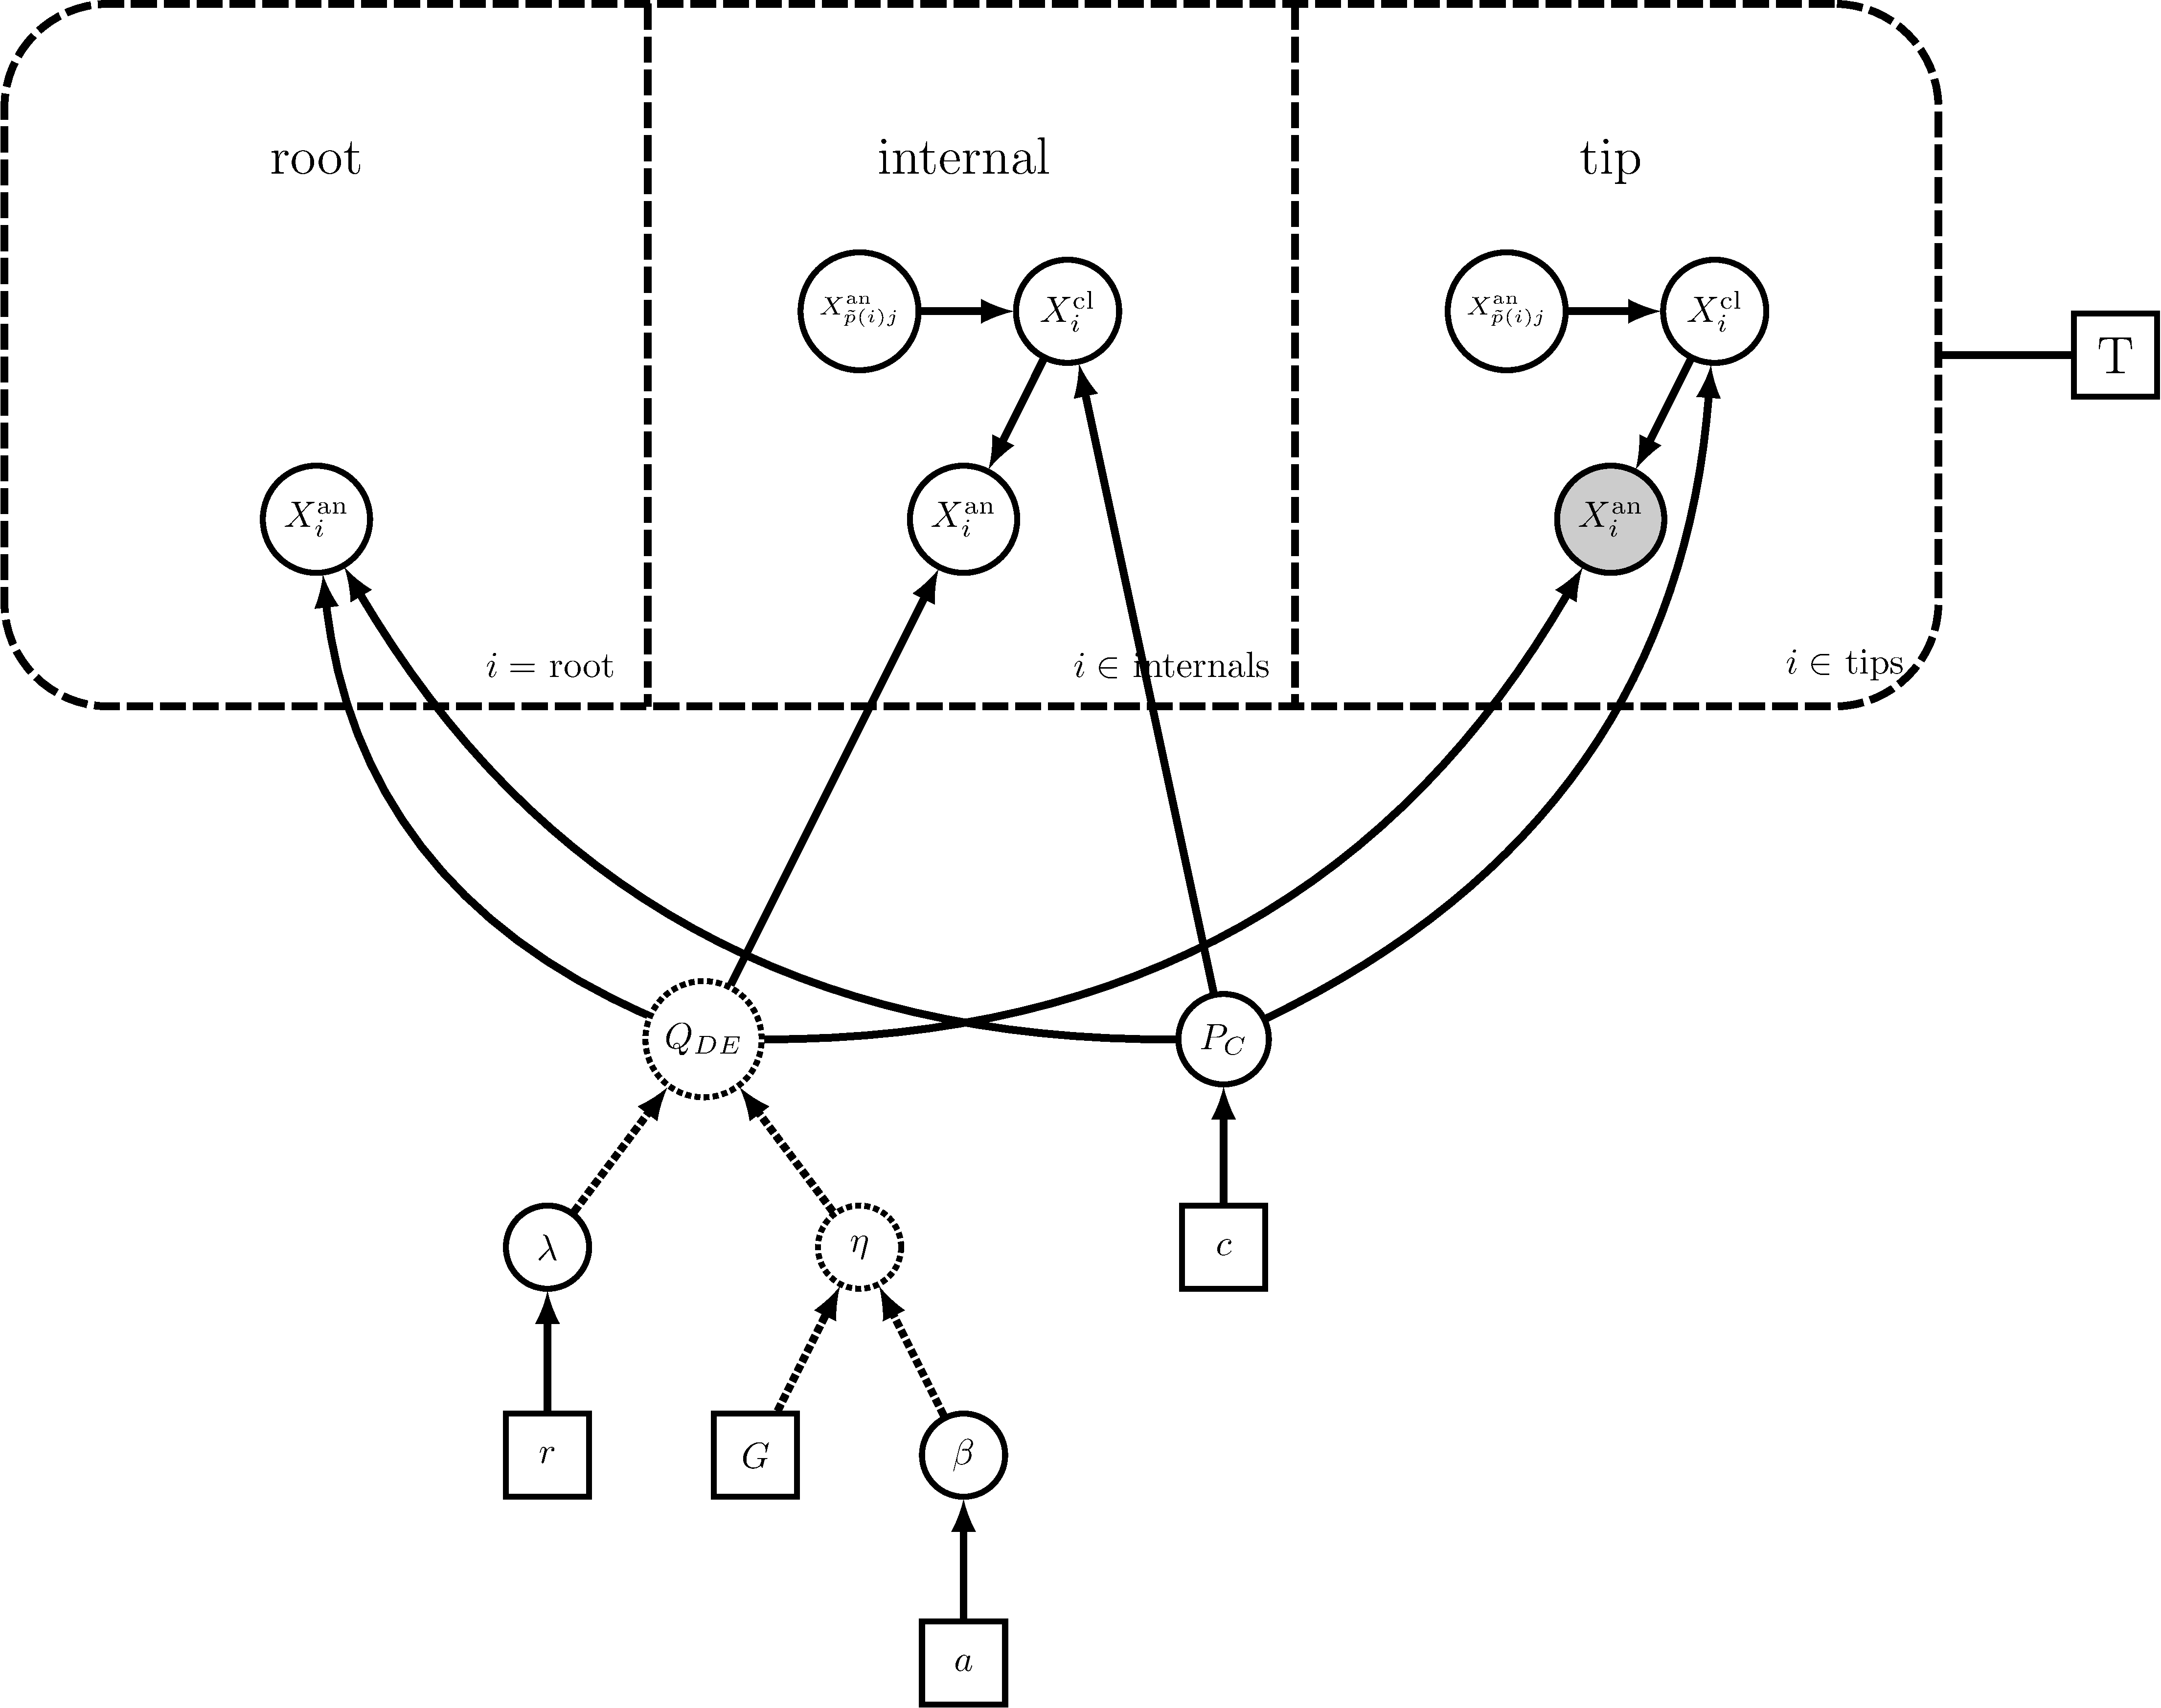
\includegraphics[width=5in]{figures/bg_dec_dag}
\caption{Graphical model of DEC. The tree plate's topology is fixed by $T$, where each internal node has both an anagenic and cladogenic random variable ($X_i^{\text{an}}$ and $X_i^{\text{cl}}$, resp.) that represents an ancestral species before and after it speciated. Anagenic change is modeled by a continuous time Markov process, where $Q_{DE}$ is the instantaneous rate matrix of area gain and loss, as parameterized by $\lambda$. The geographic distance rate modifier function, $\eta$, takes in the geographical distances and strata as $G$, and the distance power parameter, $\beta$. Cladogenic change is modeled by $P_C$, a Dirichlet-distributed simplex with a flat prior.}
\end{figure}

The rest of this tutorial will describe how to assemble the input, run the analysis, assess the output, and visualize the results.

\newpage

%%%%%%%%%%%%%%%%
%%%%%%%%%%%%%%%%
\subsection{Input}

For this tutorial, we'll use a dataset for 19 species of $Psychotria$ whose range spans the Hawaiian archipelago.
The dataset was originally reported in \citet{nepokroeff03} and analyzed using the maximum likelihood method, LAGRANGE, by \citet{ree08}.
We'll use this dataset for three reasons.
First, it is relatively small, meaning we can produce results quickly.
Second, the Hawaiian archipelago can be broken into naturally discrete areas and has a well-characterized geographical history that is uncomplicated to model.
Third, it has previously been analyzed, which provides some basis for comparison to other methods.
To simplify things, this model will assume we live in a gentler world where presence-absence characters are known without error.

For larger datasets to play with, see {\tt input/sim\_aus\_50tip\_33area.*} for a simulated model where all cladogenic events were sympatric (wide and narrow only). 


\subsection{RevBayes Analysis}

There are six major parts to the analysis.

First, we need to read in the input files and assign analysis settings.
Second, we need to construct our model.
Third, we need to assign moves and monitors to our model parameters for use with Markov chain Monte Carlo (MCMC).
Fourth, we will run an MCMC analysis assuming a complex model.
Fifth, we will compare the complex model with a simple model using Bayes factors.
Finally, we'll analyze our MCMC output.


\bibliography{bayes}